% Qwen3-8B task scores, copied verbatim from main.tex / tab:qwen_results.
% Axis order: HotPotQA, IFBench, HoVer, PUPA, AIME-2025, LiveBench-Math.
% Each spoke has an explicitly labeled linear score range (center to rim).
% Axis-local zoom changes geometry only; the 36 raw scores are unchanged.
% Native-size vector graphic: 67 mm wide; labels are 8.5 pt before inclusion.
\documentclass[tikz,border=0pt]{standalone}
\usepackage[T1]{fontenc}
\usepackage{newtxtext,newtxmath}
\usetikzlibrary{plotmarks}

\definecolor{seed}{HTML}{7D858C}
\definecolor{grpo}{HTML}{009E73}
\definecolor{mipro}{HTML}{9B639D}
\definecolor{gepa}{HTML}{0072B2}
\definecolor{merge}{HTML}{56B4E9}
\definecolor{compass}{HTML}{D55E00}
\definecolor{grid}{HTML}{DDE2E7}
\definecolor{ink}{HTML}{303840}

\tikzset{
  seed/.style={draw=seed, densely dotted, line width=0.55pt,
    mark=o, mark size=1.25pt, mark options={solid, fill=white}},
  grpo/.style={draw=grpo, dashed, line width=0.65pt,
    mark=triangle*, mark size=1.4pt, mark options={solid, fill=white}},
  mipro/.style={draw=mipro, dash pattern=on 3pt off 1.5pt,
    line width=0.65pt, mark=square*, mark size=1.2pt,
    mark options={solid, fill=white}},
  gepa/.style={draw=gepa, line width=0.8pt, mark=diamond*,
    mark size=2.0pt, mark options={solid, fill=white}},
  merge/.style={draw=merge, dash pattern=on 4pt off 1.5pt on 0.8pt off 1.5pt,
    line width=0.7pt, mark=x, mark size=1.5pt, mark options={solid}},
  compass/.style={draw=compass, line width=1.25pt, mark=*,
    mark size=1.6pt, mark options={solid, fill=compass}},
  label/.style={font=\rmfamily\fontsize{8.5}{9.2}\selectfont, text=ink, inner sep=1pt},
  axisrange/.style={font=\rmfamily\fontsize{8.5}{9.2}\selectfont, text=seed, inner sep=1pt},
}

% Ranges include every method, with margin on both ends.
\def\axismin{{40,25,30,75,15,40}}
\def\axismax{{70,45,60,95,75,80}}
\newcommand{\radardata}[2]{%
  \foreach \value [count=\i] in {#2}{%
    \pgfmathsetmacro{\angle}{90-60*(\i-1)}%
    \pgfmathsetmacro{\lo}{\axismin[\i-1]}%
    \pgfmathsetmacro{\hi}{\axismax[\i-1]}%
    \pgfmathsetmacro{\radius}{1.78*(\value-\lo)/(\hi-\lo)}%
    \coordinate (#1-\i) at (\angle:\radius);
  }%
}
\newcommand{\radarline}[1]{%
  \draw[#1] (#1-1)--(#1-2)--(#1-3)--(#1-4)--(#1-5)--(#1-6)--cycle;
}
\newcommand{\radarmarks}[1]{%
  \foreach \i in {1,...,6}{%
    \path plot[only marks,#1] coordinates {(#1-\i)};
  }%
}
\newcommand{\legendentry}[4]{%
  \draw[#1] (#2,#3)--++(0.48,0);
  \path plot[only marks,#1] coordinates {(#2+0.24,#3)};
  \node[label,anchor=west] at (#2+0.58,#3) {#4};
}

\begin{document}
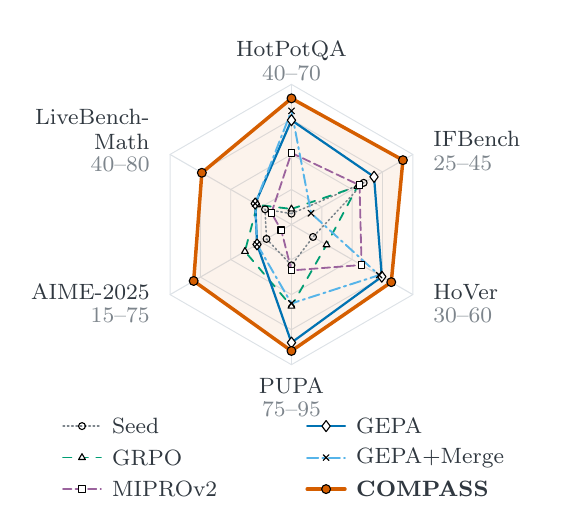
\begin{tikzpicture}[line cap=round, line join=round]
\path[use as bounding box] (-3.35,-3.05) rectangle (3.35,3.00);
\begin{scope}[yshift=0.50cm]
  \foreach \level in {25,50,75,100}{
    \pgfmathsetmacro{\r}{1.78*\level/100}
    \draw[grid,line width=0.35pt]
      (90:\r)--(30:\r)--(-30:\r)--(-90:\r)--(-150:\r)--(150:\r)--cycle;
  }
  \foreach \angle in {90,30,-30,-90,-150,150}{
    \draw[grid,line width=0.4pt] (0,0)--(\angle:1.78);
  }

  \radardata{seed}{42.33,36.90,35.33,80.82,27.33,48.70}
  \radardata{grpo}{43.33,35.88,38.67,86.66,38.00,51.26}
  \radardata{mipro}{55.33,36.22,47.33,81.55,20.00,46.60}
  \radardata{gepa}{62.33,38.61,52.33,91.85,32.00,51.95}
  \radardata{merge}{64.33,28.23,51.67,86.26,32.00,51.95}
  \radardata{compass}{67.00,43.37,54.67,93.04,63.33,69.53}

  \path[fill=compass,fill opacity=0.075]
    (compass-1)--(compass-2)--(compass-3)--(compass-4)--(compass-5)--(compass-6)--cycle;
  \foreach \series in {seed,grpo,mipro,gepa,merge,compass}{\radarline{\series}}
  \foreach \series in {seed,grpo,mipro,gepa,merge,compass}{\radarmarks{\series}}

  \node[label,anchor=south] at (0,2.04) {HotPotQA};
  \node[axisrange,anchor=north] at (0,2.05) {40--70};
  \node[label,anchor=west] at (1.76,1.09) {IFBench};
  \node[axisrange,anchor=west] at (1.76,0.78) {25--45};
  \node[label,anchor=west] at (1.76,-0.85) {HoVer};
  \node[axisrange,anchor=west] at (1.76,-1.16) {30--60};
  \node[label,anchor=north] at (0,-1.91) {PUPA};
  \node[axisrange,anchor=north] at (0,-2.21) {75--95};
  \node[label,anchor=east] at (-1.76,-0.85) {AIME-2025};
  \node[axisrange,anchor=east] at (-1.76,-1.16) {15--75};
  \node[label,anchor=east,align=right] at (-1.76,1.21) {LiveBench-\\Math};
  \node[axisrange,anchor=east] at (-1.76,0.76) {40--80};
\end{scope}

\legendentry{seed}{-2.90}{-2.06}{Seed}
\legendentry{grpo}{-2.90}{-2.46}{GRPO}
\legendentry{mipro}{-2.90}{-2.86}{MIPROv2}
\legendentry{gepa}{0.20}{-2.06}{GEPA}
\legendentry{merge}{0.20}{-2.46}{GEPA+Merge}
\legendentry{compass}{0.20}{-2.86}{\textbf{COMPASS}}
\end{tikzpicture}
\end{document}
